\section{Evaluation}
\label{sec:evaluation}

\subsection{Logging Window}
\emph{Watt's Happening} selected a five minute logging window.
This window was chosen to balance impact on the system with a desire to capture as much data as possible, as mentioned in Section \ref{subsec:impl_logging}.
Our timing window also impacts our time remaining calculation, described in Section %TODO citation 
As we've seen in our test cases, because battery level does not change for long periods of time while the phone idles, shorter logging windows would not provide more utility for our estimations. %TODO table ref
Using less than a five minute window, the number of short term observations with no battery change registered will grow, which results in more logging with no gain in useful data.
If more fine-grained battery information is required, we could register a \texttt{BatteryLevelChange} event handler to capture exactly when a battery level change occurs.
If we extend the logging window, there is a higher chance of missing applications that impact battery depletion.

\subsection{Estimation Model}
Initially, we experimented with using long term historical usage metrics in estimating application resource consumption.
This led to overestimation, since usage spikes are overly smoothed into long periods of near-zero resource consumption.
%This led to overestimation, since current usage is overly smoothed.
Next, we attempted to incorporate both long and short term usage metrics in estimating application resource consumption by doing a weighted average.
While our estimates improved, this still resulted in overestimation. 
Both overestimations were due to long periods with a lower rate of battery use outweighing short periods with a higher rate of battery use, that could continue until the end of the battery.
%This led to overestimation, since long periods with a lower rate of battery use outweighed the short periods with a higher rate of battery use that could continue until the end of the battery.
Due to our goal of not overestimating remaining battery levels, our estimation is derived primarily from short term use when available and falling back on historic usage information, as described in Section \ref{subsec:impl_analysis}.

\subsection{Experimentation}
% Methodology
Although formal and repeatable testing would have provided a consistent and controlled environment to display incontrovertible usage trends, a sterile environment is not the expected use case.
Therefore, averaging real world usage scenarios provide a more realistic, yet hopefully still convincing, data set.
\emph{Watt's Happening} was tested and analyzed via iterative real world testing on a selection of Android devices for over 40 hours of total testing time.
The devices include an HTC EVO 3D and a Motorola Droid RAZR both running Android 4.0. 

\subsection{Performance}
\begin{figure*}[h]
	\begin{center}
		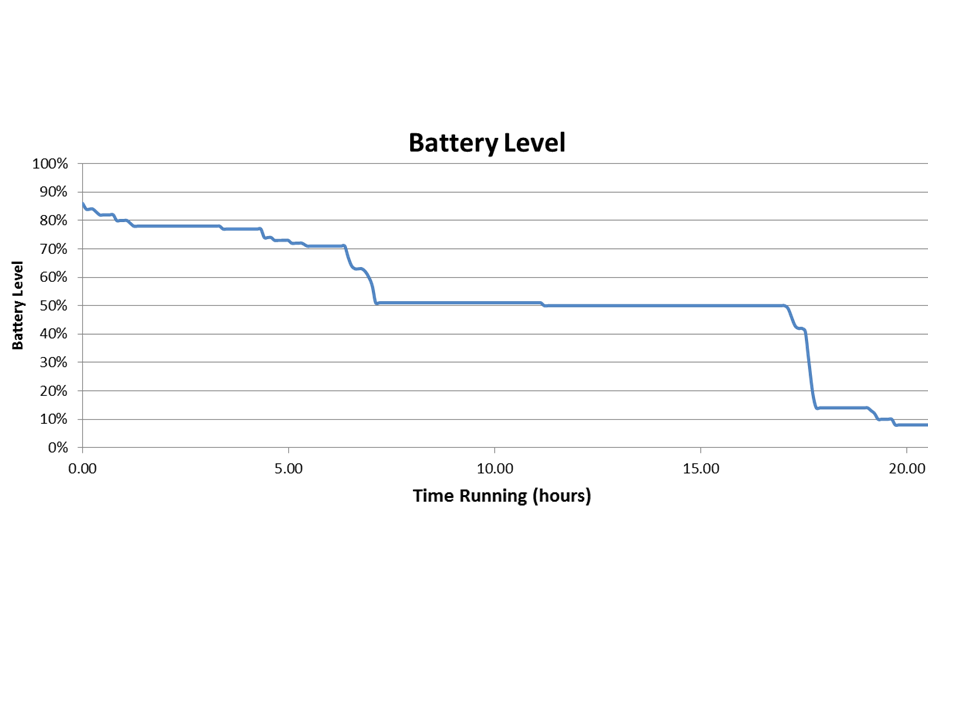
\includegraphics[scale=0.5]{figs/battery_level.png}
		\caption{Battery Level Over Time, Dataset 1}
		\label{fig:bat_level}
\end{center}
\end{figure*}
\begin{figure*}[h]
	\begin{center}
		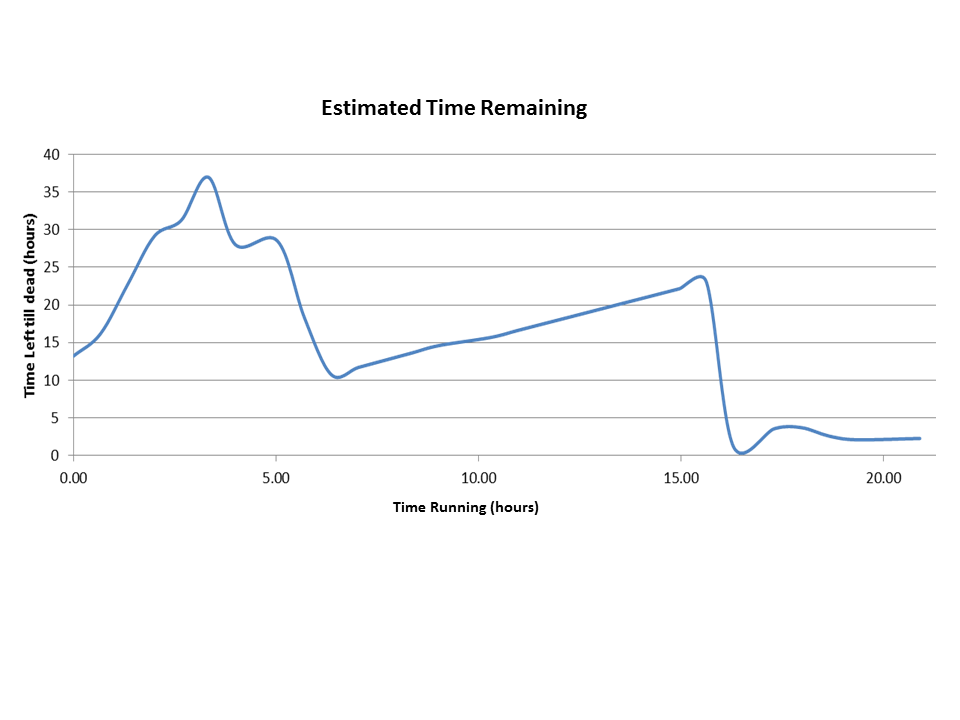
\includegraphics[scale=0.5]{figs/est_time_remaining.png}
		\caption{Estimated Time Remaining Over Time, Dataset 1}
		\label{fig:est_remaining}
\end{center}
\end{figure*}
\begin{figure*}[h]
	\begin{center}
		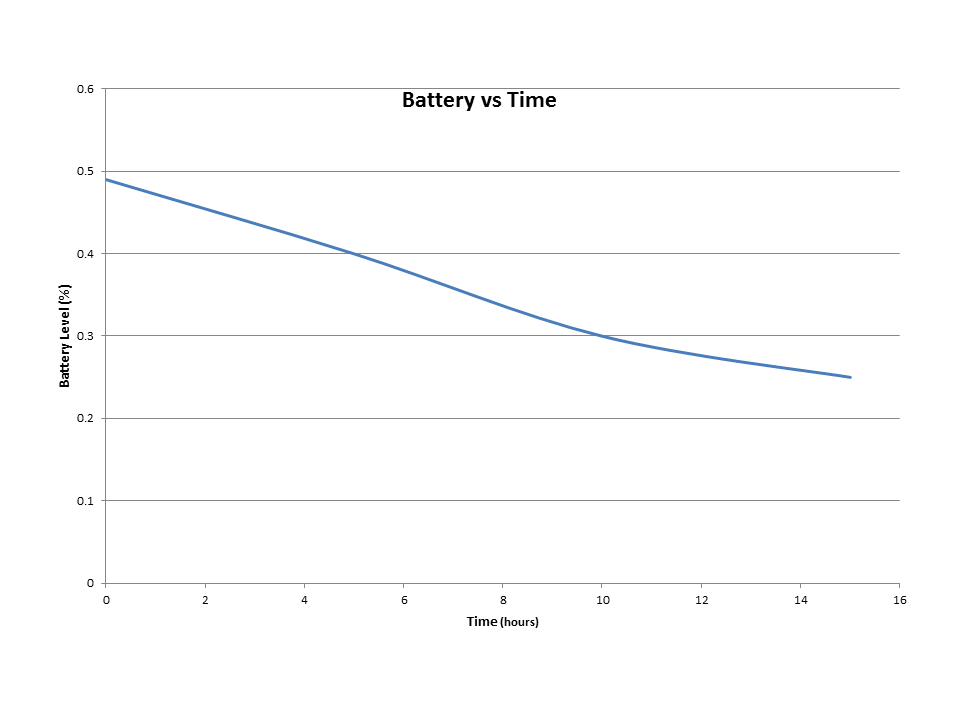
\includegraphics[scale=0.5]{figs/bat_vs_time_short.png}
		\caption{Battery Level Over Time, Dataset 2}
		\label{fig:bat_vs_time_short}
\end{center}
\end{figure*}
Figure \ref{fig:bat_level} shows the battery depletion over an approximately 20 hour run, beginning at approximately 11:00am. 
The long period of minimal battery depletion aligns with our test user's sleeping habits.
A sharp spike of device usage and corresponding battery depletion is evident, and correlates to our test user streaming music over 3G, a relatively resource intensive task.


Figure \ref{fig:est_remaining} is from the same test period as figure \ref{fig:bat_level}.
This figure shows \emph{Watt's Happening}'s estimate of remaining battery time, calculated every 30 minutes.
As we can see, over long idle periods our estimation tends to increase.
Conversely, over periods of heavy use, our estimation dramatically decreases in correlation with recent high usage.
%TODO softshoe around overestimation
Figure \ref{fig:bat_vs_time_short} shows the battery depletion over a 15 minute run.
The battery level drops from 50\% to 25\% over only 15 minutes, corresponding to our test user's use of a CPU-intensive game (in this case, \emph{Great Little War Game}\cite{glwg}).
At the end of this use session, Watt's Happening estimates that approximately 25 minutes of battery life remains if application use is continued.
This estimate is accurate, assessed by our test user and drawing from his past observations and experience.
%TODO- Nick is going to run his phone into the ground so we don't have to sound wishy-washy

Since the goal of \emph{Watt's Happening} is to monitor application resource usage, we can use  \emph{Watt's Happening} to monitor itself.
In our test runs, \emph{Watt's Happening} routinely uses a negligible amount of CPU resources, in relation to other running applications.
Therefore, we conclude that the resource consumption of \emph{Watt's Happening} is acceptable.
Although we the developers of \emph{Watt's Happening} have taken great strides toward conservative yet accurate battery life estimates, runs with long idle times may still have some amount of overestimation.
%
When taken in context to the life of the universe, for example, over estimation by hours is a very small thing. 
Humans don't live that long, anyway.
Timey-Wimey   %that got away from you there
%
This is due to the averaging of historic data.  
Potential solutions include removing long periods of idle time from the averaged data or using exponential weighted moving averages to deemphasize periods of low use the further these periods are from the present.

